 

\chapter[Change of variables \texorpdfstring{\normalfont  $\textrm{d}x_i = -\mathbf{N}^T \mathbf{d}_i \textrm{d}x/z_i^3$}{}]{Change of variables \\ \texorpdfstring{\normalfont $\textrm{d}x_i = -\mathbf{N}^T \mathbf{d}_i \textrm{d}x/z_i^3$}{}}
\label{app:change}

In the photometric refinement step we derived a simplified expression for the gradient computetion, thanks to the change of variables:
\begin{equation}
 \textrm{d}x_i = -\mathbf{N}^T \mathbf{d}_i \textrm{d}x/z_i^3
\end{equation}
which is well-known in literature, and usually its derivation is omitted.
We report here the complete derivation of the formula.

The idea behind this change of variables is the expression of the variation of the solid angle subtended by the 3D surface and by the image. 
In both case we rely on the relation:
\begin{equation}
    \omega = \frac{A}{r^2},
\end{equation}
where $A$ is the area the angle is subtended by and $r$ is the radius from the center to the area.


\begin{figure}[bt]
 \centering
 \begin{tabular}{c}
  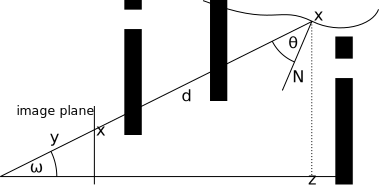
\includegraphics[width=0.8\textwidth]{./img/ch-appendix/change01}\\
 \end{tabular}
 \caption{Variables involved in the computations.}
 \label{fig:change}
\end{figure}

 
Let express how the variation of point $\mathbf{x}$ on the 3D surface $\mathbb{S}$ affects the angle $\omega$ (see Figure \ref{fig:change}):
\begin{equation}
    d\omega = \frac{dA}{\mathbf{d}_i^2} = \frac{\cos(\theta)}{\mathbf{d}_i^2}d\mathbf{x}.
\end{equation}
By expressing $\cos(\theta) = -\frac{\mathbf{N^T x}}{\mathbf{d}_i}$,  we rewrite:
\begin{equation}
\label{eq:change1}
    d\omega  = -\frac{\mathbf{N^T x}}{\mathbf{d}_i^3}d\mathbf{x}.
\end{equation}

Similarly we can express the variation of the point $\mathbf{x}_i$ on the image as: 
\begin{equation}
    d\omega = \frac{dA}{\mathbf{d}_i^2} = \frac{\cos(\theta)}{\mathbf{d}_i^2}d\mathbf{x}.
\end{equation}

\begin{equation}
\label{eq:change2}
    d\omega = \frac{dA}{\mathbf{d}_i^2} = \frac{\cos(\alpha)}{|\mathbf{x}_i|^2}d\mathbf{x}_i.
\end{equation}
By expressing $\cos(\alpha) = \frac{f}{|\mathbf{x}_i|}$,  we rewrite:
\begin{equation}
    d\omega  = -\frac{f}{|\mathbf{x}_i|^3}d\mathbf{x}_i.
\end{equation}
Since
\begin{equation}
 \frac{|\mathbf{d}_i|}{|\mathbf{x}_i|} = \frac{f}{z_i^3},
\end{equation}
Equation \eqref{eq:change2} becomes:
\begin{equation}
\label{eq:change3}
    d\omega  = \frac{z_i^3}{|\mathbf{d}_i|^3 f^2}d\mathbf{x}_i.
\end{equation}

Finally, we derive the change of variable by substituting \eqref{eq:change3} in  \eqref{eq:change1}:


\begin{equation}
\label{eq:change4}
    \frac{z_i^3}{|\mathbf{d}_i|^3 f^2}d\mathbf{x}_i = -\frac{\mathbf{N^T x}}{\mathbf{d}_i^3}d\mathbf{x}.
\end{equation}

\begin{equation}
\label{eq:change5}
    d\mathbf{x}_i = -\frac{f^2 \mathbf{N^T x}}{z_i^3}d\mathbf{x}.
\end{equation}



